% Chapter 3

\chapter{Materials} % Main chapter title

\label{Materials} % For referencing the chapter elsewhere, use \ref{Materials} 


%----------------------------------------------------------------------------------------
\section{Infectious clone of MVMp (pIC\_MVMp)}
\label{IC}


\subsection{Plasmid map of pIC\_MVMp}

\begin{figure}[h] 
\begin{center}
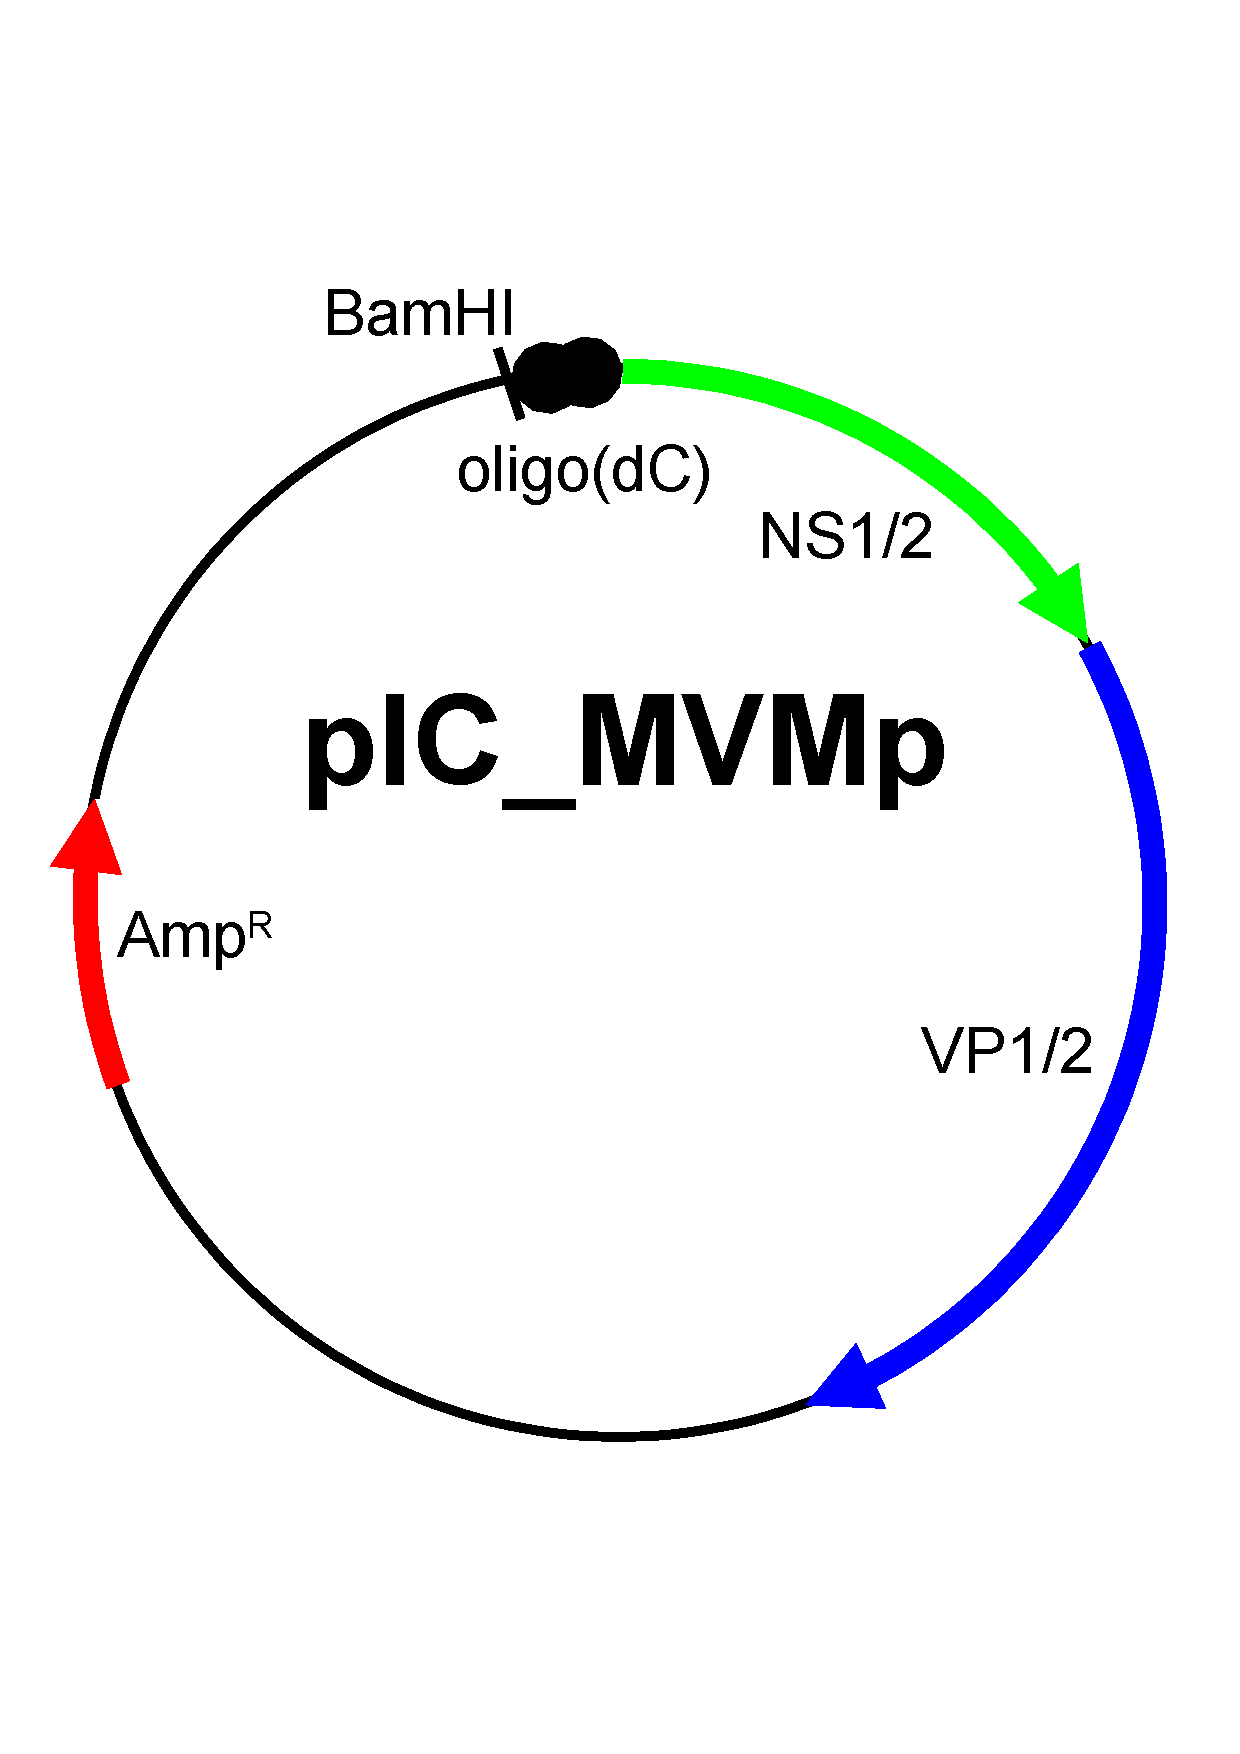
\includegraphics[width=0.5\textwidth]{pIC_MVMp}
\caption[Plasmid map of the infectious clone of MVMp]{Plasmid map of the infectious clone of MVM (pIC\_MVMp). Colored arrows indicate the genes in either the MVMp genome or the pBR322 cloning vector. The circles at the left-hand end of the MVM genome represent the oligo(dC) linker sequence which was originally used for cloning \cite{pmid6345805}.}
\label{pIC}
\end{center}
\end{figure}

\subsection{Complete sequence of pIC\_MVMp}
\label{sequence}

\raggedright
The complete sequence of the infectious clone of MVM (pIC\_MVMp) is shown below. Sequences in black correspond to the backbone of the pBR322 cloning vector. The sequence colored red corresponds to the viral negative (-) strand in 3' to 5' direction which is predominantly packaged into MVM capsids.  


\begin{addmargin}{0.1\textwidth}

  \begin{footnotesize}
\begin{LVerbatim}[commandchars=\\\{\}]

   1 AAGAACTTCT GCTTTCCCGG AGCACTATGC GGATAAAAAT ATCCAATTAC AGTACTATTA 
  61 TTACCAAAGA ATCTGCAGTC CACCGTGAAA AGCCCCTTTA CACGCGCCTT GGGGATAAAC 
 121 AAATAAAAAG ATTTATGTAA GTTTATACAT AGGCGAGTAC TCTGTTATTG GGACTATTTA 
 181 CGAAGTTATT ATAACTTTTT CCTTCTCATA CTCATAAGTT GTAAAGGCAC AGCGGGAATA 
 241 AGGGAAAAAA CGCCGTAAAA CGGAAGGACA AAAACGAGTG GGTCTTTGCG ACCACTTTCA 
 301 TTTTCTACGA CTTCTAGTCA ACCCACGTGC TCACCCAATG TAGCTTGACC TAGAGTTGTC 
 361 GCCATTCTAG GAACTCTCAA AAGCGGGGCT TCTTGCAAAA GGTTACTACT CGTGAAAATT 
 421 TCAAGACGAT ACACCGCGCC ATAATAGGGC ACAACTGCGG CCCGTTCTCG TTGAGCCAGC 
 481 GGCGTATGTG ATAAGAGTCT TACTGAACCA ACTCATGAGT GGTCAGTGTC TTTTCGTAGA 
 541 ATGCCTACCG TACTGTCATT CTCTTAATAC GTCACGACGG TATTGGTACT CACTATTGTG 
 601 ACGCCGGTTG AATGAAGACT GTTGCTAGCC TCCTGGCTTC CTCGATTGGC GAAAAAACGT 
 661 GTTGTACCCC CTAGTACATT GAGCGGAACT AGCAACCCTT GGCCTCGACT TACTTCGGTA 
 721 TGGTTTGCTG CTCGCACTGT GGTGCTACGG ACGTCGTTAC CGTTGTTGCA ACGCGTTTGA 
 781 TAATTGACCG CTTGATGAAT GAGATCGAAG GGCCGTTGTT AATTATCTGA CCTACCTCCG 
 841 CCTATTTCAA CGTCCTGGTG AAGACGCGAG CCGGGAAGGC CGACCGACCA AATAACGACT 
 901 ATTTAGACCT CGGCCACTCG CACCCAGAGC GCCATAGTAA CGTCGTGACC CCGGTCTACC 
 961 ATTCGGGAGG GCATAGCATC AATAGATGTG CTGCCCCTCA GTCCGTTGAT ACCTACTTGC 
1021 TTTATCTGTC TAGCGACTCT ATCCACGGAG TGACTAATTC GTAACCATTG ACAGTCTGGT 
1081 TCAAATGAGT ATATATGAAA TCTAACTAAA TTTTGAAGTA AAAATTAAAT TTTCCTAGAT 
1141 CCACTTCTAG GAAAAACTAT TAGAGTACTG GTTTTAGGGA ATTGCACTCA AAAGCAAGGT 
1201 GACTCGCAGT CTGGGGCATC TTTTCTAGTT TCCTAGAAGA ACTCTAGGAA AAAAAGACGC 
1261 GCATTAGACG ACGAACGTTT GTTTTTTTGG TGGCGATGGT CGCCACCAAA CAAACGGCCT 
1321 AGTTCTCGAT GGTTGAGAAA AAGGCTTCCA TTGACCGAAG TCGTCTCGCG TCTATGGTTT 
1381 ATGACAGGAA GATCACATCG GCATCAATCC GGTGGTGAAG TTCTTGAGAC ATCGTGGCGG 
1441 ATGTATGGAG CGAGACGATT AGGACAATGG TCACCGACGA CGGTCACCGC TATTCAGCAC 
1501 AGAATGGCCC AACCTGAGTT CTGCTATCAA TGGCCTATTC CGCGTCGCCA GCCCGACTTG 
1561 CCCCCCAAGC ACGTGTGTCG GGTCGAACCT CGCTTGCTGG ATGTGGCTTG ACTCTATGGA 
1621 TGTCGCACTC GATACTCTTT CGCGGTGCGA AGGGCTTCCC TCTTTCCGCC TGTCCATAGG 
1681 CCATTCGCCG TCCCAGCCTT GTCCTCTCGC GTGCTCCCTC GAAGGTCCCC CTTTGCGGAC 
1741 CATAGAAATA TCAGGACAGC CCAAAGCGGT GGAGACTGAA CTCGCAGCTA AAAACACTAC 
1801 GAGCAGTCCC CCCGCCTCGG ATACCTTTTT GCGGTCGTTG CGCCGGAAAA ATGCCAAGGA 
1861 CCGGAAAACG ACCGGAAAAC GAGTGTACAA GAAAGGACGC AATAGGGGAC TAAGACACCT 
1921 ATTGGCATAA TGGCGGAAAC TCACTCGACT ATGGCGAGCG GCGTCGGCTT GCTGGCTCGC 
1981 GTCGCTCAGT CACTCGCTCC TTCGCCTTCT CGCGGACTAC GCCATAAAAG AGGAATGCGT 
2041 AGACACGCCA TAAAGTGTGG CGTATACCAC GTGAGAGTCA TGTTAGACGA GACTACGGCG 
2101 TATCAATTCG GTCATATGTG AGGCGATAGC GATGCACTGA CCCAGTACCG ACGCGGGGCT 
2161 GTGGGCGGTT GTGGGCGACT GCGCGGGACT GCCCGAACAG ACGAGGGCCG TAGGCGAATG 
2221 TCTGTTCGAC ACTGGCAGAG GCCCTCGACG TACACAGTCT CCAAAAGTGG CAGTAGTGGC 
2281 TTTGCGCGCT CCGTCGACGC CATTTCGAGT AGTCGCACCA GCACTTCGCT AAGTGTCTAC 
2341 AGACGGACAA GTAGGCGCAG GTCGAGCAAC TCAAAGAGGT CTTCGCAATT ACAGACCGAA 
2401 GACTATTTCG CCCGGTACAA TTCCCGCCAA AAAAGGACAA ACCAGTGAAC TACGGAGGCA 
2461 CATTCCCCCT TAAAGACAAG TACCCCCATT ACTATGGCTA CTTTGCTCTC TCCTACGAGT 
2521 GCTATGCCCA ATGACTACTA CTTGTACGGG CCAATGACCT TGCAACACTC CCATTTGTTG 
2581 ACCGCCATAC CTACGCCGCC CTGGTCTCTT TTTAGTGAGT CCCAGTTACG GTCGCGAAGC 
2641 AATTATGTCT ACATCCACAA GGTGTCCCAT CGGTCGTCGT AGGACGCTAC GTCTAGGCCT 
2701 TGTATTACCA CGTCCCGCGA CTGAAGGCGC AAAGGTCTGA AATGCTTTGT GCCTTTGGCT 
2761 TCTGGTAAGT ACAACAACGA GTCCAGCGTC TGCAAAACGT CGTCGTCAGC GAAGTGCAAG 
2821 CGAGCGCATA GCCACTAAGT AAGACGATTG GTCATTCCGT TGGGGCGGTC GGATCGGCCC 
2881 AGGAGTTGCT GTCCTCGTGC TAGTACGCGT GGGCACCGGT CCTGGGTTGC GACGGGCTCT 
2941 ACGCGGCGCA CGCCGACGAC CTCTACCGCC TGCGCTACCT ATACAAGACG GTTCCCAACC 
3001 AAACGCGTAA GTGTCAAGAG GCGTTCTTAA CTAACCGAGG TTAAGAACCT CACCACTTAG 
3061 GCAATCGCTC CACGGCGGCC GAAGGTAAGT CCAGCTCCAC CGGGCCGAGG TACGTGGCGC 
3121 TGCGTTGCGC CCCTCCGTCT GTTCCATATC CCGCCGCGGA TGTTAGGTAC GGTTGGGCAA 
3181 GGTACACGAG CGGCTCCGCC GTATTTAGCG GCACTGCTAG TCGCCAGGTC ACTAGCTTCA 
3241 ATCCGACCAT TCTCGGCGCT CGCTAGGAAC TTCGACAGGG ACTACCAGCA GTAGATGGAC 
3301 GGACCTGTCG TACCGGACGT TGCGCCCGTA GGGCTACGGC GGCCTTCGCT CTTCTTAGTA 
3361 TTACCCCTTC CGGTAGGTCG GAGCGCAGCG CTTGCGGTCG TTCTGCATCG GGTCGCGCAG 
3421 CCGGCGGTAC GGCCGCTATT ACCGGACGAA GAGCGGCTTT GCAAACCACC GCCCTGGTCA 
3481 CTGCTTCCGA ACTCGCTCCC GCACGTTCTA AGGCTTATGG CGTTCGCTGT CCGGCTAGTA 
3541 GCAGCGCGAG GTCGCTTTCG CCAGGAGCGG CTTTTACTGG GTCTCGCGAC GGCCGTGGAC 
3601 AGGATGCTCA ACGTACTATT TCTTCTGTCA GTATTCACGC CGCTGCTATC AGTACGGGGC 
3661 GCGGGTGGCC TTCCTCGACT GACCCAACTT CCGAGAGTTC CCGTAGCCAG CTGCGAGAGG 
3721 GAATACGCTG AGGACGTAAT CCTTCGTCGG GTCATCATCC AACTCCGGCA ACTCGTGGCG 
3781 GCGGCGTTCC TTACCACGTA CGTTCCTCTA CCGCGGGTTG TCAGGGGGCC GGTGCCCCGG 
3841 ACGGTGGTAT GGGTGCGGCT TTGTTCGCGA GTACTCGGGC TTCACCGCTC GGGCTAGAAG 
3901 GGGTAGCCAC TACAGCCGCT ATATCCGCGG TCGTTGGCGT GGACACCGCG GCCACTACGG 
3961 CCGGTGCTAC GCAGGCCGCA TCTCCTAGGC CCCCCCCCCC CCC\color{red}AAAATCT TGACTGGTTG 
\color{red}4021 GTACAAGTGC ATTCACTGCA CTACTGCGCG CGACGCGCGC GACGGAAGCC GTCAGTGTGC 
\color{red}4081 AGTGAATGCA AAGTGTACCA ACCAGTCAAG ATTTTTACTA TTCGCCAAGT CCCTCAAATT 
\color{red}4141 TGGTTCCGCG CTTTTCCTTC ACCCGCACCA AATTTCATAT ATTCGTTGAT GACTTCAGTC 
\color{red}4201 AATGAATAGA AAAGAAAGTA AGACACTCAG CTCTGCGTGT CTTTCTCTCA TTGGTTGATT 
\color{red}4261 GGTACCGACC TTTACGAATG AGACTACTTC AAAACCCTCG TTGGTTGACC AATTTCCTTT 
\color{red}4321 TTTCATTGGT CCTTCACAAG AGTAAACAAA AATTTTTACT TTTACAAGTT GACTTACCTT 
\color{red}4381 TTCTATAGCC TACCTTATCA ATGTTTTTTC TCGACGTCCT CCTGCTCGAC TTTAGAAATG 
\color{red}4441 TTGCTCCTCG CCTTTGATGA ACCCTGGTTT CGCTCCTGTA CCTTACCCTT TGGTGTCACC 
\color{red}4501 TACTTTACTG GTTTTTCGTT CATAAGTAAA AACTAAGAAA CCAATTTTTT ACAAATAAAC 
\color{red}4561 TTCACGAATT GTGTTTCTTA TATAAAGGAC CACTACAATT AACCAAACAC GTTGTACTTA 
\color{red}4621 CCCCTTTTCT GGTTCCGACC GTGACGGTAC ATGATTAACC TCCTTTCCTG AAATCAGTTC 
\color{red}4681 GAGTTCCCTT TACCACCTCT TCCGTTGATT TACAAATGAC CTCGTCTACC AACCATTGTC 
\color{red}4741 GGACATTACA CGTTGATTGT GGTCGACTTT CTTAATTTGA TTCTCTTTAT CGTCTTCTGT 
\color{red}4801 TACTCACCCA ATGAGATGAA TGAATATTCG TATTCGTTTG GTTTTTTCTG ATATGGTTCA 
\color{red}4861 CACAAGAAAA ACCTTTGTAC TAACGAATGA TAAAAAATTG ATTTTTCTTT TATTCGTGAT 
\color{red}4921 CAGGTGGTTC TCTGCCTCCG ATAAAAGAAA TCGTCACTGA AACCGACCTT TTGATTGAAA 
\color{red}4981 AATTTTCTTC CGCTCGCGGT AGATCACTCG TTTGATATGT GACTACTGTA CGCCGGTCTT 
\color{red}5041 TGCCAACTTT GGTGTCATTG GTGACGCGTC CTTTGATTCG CGCCGTCTTA AGTTTGATTT 
\color{red}5101 TTTCTTCAAA GATAATTTTG ATGTGAATTT CTCGACCACG TATTTTCTCA TTGGAGTGGT 
\color{red}5161 CTCCTGACCT ACTACTACGT CGGTCTGTCA ATGTAACTTT ACTACCGAGT TGGTCCACCT 
\color{red}5221 CTTTTGGACG ACTTTTTATG CGATCTCTAA ACATGTGATT GAGATCGGTC TTGGTTTTGT 
\color{red}5281 CGTAAACTGA ATTAAAATCT TTTTCGACTT TGGTCGTTTG ATTGGTTGAA AAGTGACGGA 
\color{red}5341 CTGTGTTCTT GGACGTCTTA AAAACGAAAA GTACCGACCT TGATACAATT TCAAACGGTA 
\color{red}5401 CGATAAACGA CACAAAATTT GTCTGTTCCT CCGTTTTCTT TATGACAAAA TAAAGTACCT 
\color{red}5461 GGTCGGTCGT GTCCGTTTAG ATAATAACGT GTTCGGTATC GTGTTCGTCA ACCGTTACAA 
\color{red}5521 CCAACGATAT TACGTCGGTT ACATTTGAAA GGTAAATTAC TGACATGGTT GTTCTTGAAC 
\color{red}5581 TAAACCCATC TTCTTCGACC ATTGAAACCT GTCGTTCATT TGGTCAAATT TCGGTAAACG 
\color{red}5641 AGACCAGTTT GATAAGCGTA ACTAGTTTTT CCTTTTCCGT CGTTTGTCTA ACTTGGTTGT 
\color{red}5701 GGTCAGTAGT ACTGGTGTTT ACTCTTGTAA TGTCACCAGT CTTATCCGAC GCTTCTTTCT 
\color{red}5761 GGTCTTGTGT GAGTTGGTTA GTCTCTGTCT TACGAATTGT AAGTAGATTG TGTATGGAAC 
\color{red}5821 GGACCACTGA AACCAAACCA ACTGTTTTTA CTTACCGGGT ACTAAACACG AACCAACCAT 
\color{red}5881 TTCTTACCAA TGGTTAGATG GTACCGTTCG ATGACACGAT TTACCCCGTT TCAAGGACTA 
\color{red}5941 ACCAGTCTTT TGACCCGCCT CGGTTTCCAC GGTTGAGGAT ATTTAAATGA TCCAAGCCGT 
\color{red}6001 GCGAGTGGTA AGTGCTGTGG CTTTTCATGC GGAGAGTCGG TCTTGATACG TGATTGAGGT 
\color{red}6061 GAACGTAGCC TAGAGCTCCT GGACCGAAAT CTCGGAACCT CGTGTGGTTT ATGAGGACAA 
\color{red}6121 CGCCCGTGAC GTCTTTGGGT CTTGTGACCC CTTCGACCAA GGTTTCGGAC GGTTCTACCA 
\color{red}6181 GTTGACTCGG GTTGAACCAG TCTCTAGCTC CTCCTAAACT CTCGCACGAA GCCACGCCTT 
\color{red}6241 GGCAACTTCT TTCTGAAGTC GCTCGGCGAC TTGAACCTGA TTCCATGCTA CCGCGGAGGT 
\color{red}6301 CGATTTTCTC GATTTTCTCC ATTCCCAAAT TCCCTACCAA CCAACCACCC CATAATTACA 
\color{red}6361 AATTAATGGA CAAAATGTCC GGACTTTAGT GAACCAAAAT CCAACCCACG GAGGACCGAT 
\color{red}6421 GTTCATGGAC CCTGGTCCCT TGTCGGAACT GGTTCCTCTT GGTTGGTTAG GTAGACTGCG 
\color{red}6481 GCGACGGTTT CTCGTGCTGC TCCGGATACT AGTTATGTAG TTTAGACCTT TTTTAGGAAT 
\color{red}6541 GGACATGAAG AGACGACGAC TAGTTGCGAA ATAACTGGTT TGGTTCCTGC GGTTTCTGAC 
\color{red}6601 CCCTCCGTTC CAACCAGTGA TGAAAAAATC TTGGTTCGCG CGAAAACGTG GATTCGAACG 
\color{red}6661 ATGACTGAGA CTTGGACCTT GAAGACCACA TTCGTCTCGA CCATTTGCGT GATCTGGTGG 
\color{red}6721 ACGAATGTAA AAATAATTGG TTCGGTCTCG ATTTTTTTTT GAATGAAGAA GACGACGTGT 
\color{red}6781 CGTTTCGTCA GTTTGGTACT CACTACCGTG GTCGGTTGGA CTGTCGCCTT TGCGACAGGT 
\color{red}6841 GAGTCGACGT TCTCAACTTG CTCGTCGACT GCCGGGACCT CCGAGACCCC CACCCCCGAG 
\color{red}6901 ACCGCCCCCA CCCCAACCAC AAAGATGACC CAGAATACTA TTAGTTTGCG TAATATCTAA 
\color{red}6961 GAACCCACTG CCGACCCATC TTTAATGACG TGATCGTTGA TCTGATCATG TAAATTTGTA 
\color{red}7021 CGGATTTAGT CTTTTGATAA CGTCTTAGTC TCAAGTGTTA TGTTGTCTGT GTAGTCAGTT 
\color{red}7081 TCCGTTGTAC CGTTTTCTAC TACGAGTACT CGTTTAAACC TGTGGTACCT CGAACCACCT 
\color{red}7141 ACGATTACGA ACCCCTCAAA CCGAGGTCGG TTCACTGACC GTTATGTAAA CGTTGTGGTA 
\color{red}7201 CTCGGTCGAA TTGAACCATA GTGAACTAGT TCTTTATAAG TTACATCACG ACTTTTGACA 
\color{red}7261 ATGTCTCGTT CTGAATCCTC CAGTTCGATA TTTTTATATG TTGTTACTGG AATGTCGAAC 
\color{red}7321 GTACTACCAA CGTCATCTGA GTTTGTTGTA AAACGGTATG TGTGGACGTC GTTTGAGTTA 
\color{red}7381 CCTTTGTGAA CCAAAGATGG GGACCTTTGG TTGGTATCGT AGTGGTATGT CCATGATAAA 
\color{red}7441 AACGCAACTG TCTCTAGAAA GTCACTGGAT GCTTTTAGTT CTTCCGTGTC AACTTGTATT 
\color{red}7501 ACACTACCCT TGTGGTTTTC CTTACTTAAG AGTTAAAAAA TGGTAACTCT TGTGTGTTGT 
\color{red}7561 TTAGTGTAAC GAGTCTTGTC CCCTGCTTAA ACGGTGTCCG TGAATGATGA AACTGTGTTT 
\color{red}7621 AGGTCAATTT GAGTGTGTGT GCACCGTTTG GTTGGCAGTT GAACCTGTCG GAGGTGACGA 
\color{red}7681 CAGTTGGAAA GGACTTCGAC TGTGACTACG TCCATGTGAA TGACGAGTTC CCTCGTCTGT 
\color{red}7741 ACCTTGTTGT GTTTACCCCC AATTGACCCA CTCACTTCGT TAGTCTTGGT CTGGACGAGT 
\color{red}7801 TCATCCTAAA ACAGTTGGTG TGGTACTGAA ACTTCGGTCG TCTCGACCTG GTAAACGACG 
\color{red}7861 GGGTTTTCAA GGTCGTCTAT AATGAGTTCC TCATCTGTTT CTTCGGTTAC CGTCACAATC 
\color{red}7921 TATGTCAATA CCGTTTGTCG TACCACTTTT AACCCGAAGT GTACCTGGTC GTGGTCTCGC 
\color{red}7981 GATGTGTACC CTACTTTGTT CGAAACCAAG TCCATCTCTG TGGTTTCTAC CAAAATAAGT 
\color{red}8041 TAGTCGTGGT GATCAACAAG GTGGTGGTGA TTTACCGTAA GAATGTTTAC GTTTGGGATA 
\color{red}8101 ACCCTGATTT TTACTGTAAG TAAAAAGTTT ACAAAAATTG TCGATACCAG GTGATTGACG 
\color{red}8161 TAAAAGTGTG GGTTCAGGAC ATATGGGAGT TCCTGTTTAT ACCCTGTTTC TTGATCTAGA 
\color{red}8221 ACTTGTGTTT GGATCTGAAG TGTATTGACG AGGTAAACAA ACATTTTTGT TACGTGGACC 
\color{red}8281 TGTTTACAAC CAATCTAATC CTGGTTTGGA TTGACTGGTT ATACTAGGTT TGCCTCGGTG 
\color{red}8341 TGAAAGATCT TAACAATGTA TACCATGTAA AAAGACCTTT CCTTTTGATT GGTACTCTCG 
\color{red}8401 TTTTGAATCT CGATTGTGGT GAACCTTGGG TCACATGGTT CATTCACGAC TTCTGTTACC 
\color{red}8461 GTTGAGTATG TACTCACATT GATTTACCGA TGGTTGACGA TGACCTTTGT ACGTCAGACA 
\color{red}8521 CGGCGAATAT TGTTCTGGAC AACGATCTTT ATGAATGATT GATTGGTACG AAAAAGAAAG 
\color{red}8581 ACATGAAGTA TATAATAATT CTGATTATTT CTATGTTGTA TCTTTATATT ATAATGTATA 
\color{red}8641 TCTAAATTCT TTATCTTATT ATACCATGAA TCATTGACAA TTTTTATTAT CTTGGAAACC 
\color{red}8701 TTATTGTTCT ATCAATCAAC CAATTACAAT CTATCTTATT CTTCTAGTAC ATATTACTTA 
\color{red}8761 TTTTCCCACC TTCCCACCAA CCATCCAATT ACAATCTATC TTATTCTTCT AGTACATATT 
\color{red}8821 ACTTATTTTC CCACCTTCCC ACCAACCATC CATAAGGGAA TCTGAACTAC AATTCCTGGT 
\color{red}8881 TTTTTTATTA TTTTGAAAAA ATTTTGAGTT GGTTCTGATG ACAGATAAGT CACTTGGTTG 
\color{red}8941 ACTTGGTAAT CATAATGATA CAAAAATCCC ACCCT\color{black}CCAGT TAGTTAGTCC TT
\end{LVerbatim}
\end{footnotesize}

\end{addmargin}






\section{Chemicals and compounds}

\begin{center}

\begin{longtable}{l l}
\textbf{Chemical} & \textbf{Provider}\\
\hline
\endfirsthead

\multicolumn{2}{l}{\textbf{Table~\ref{Chemicals}} continued}\\
\\
\textbf{Chemical} & \textbf{Provider}\\
\hline
\endhead

Acetic Acid (Glacial) & Merck\\
Acetone & Merck\\
Agarose low EEO & Applichem\\
Ampicillin (Ready Made Solution, 100 g/mL, 0.2
$\mu M$   
filtered)& Sigma-Aldrich\\
Bafilomycin A\textsubscript{1} & Sigma-Aldrich \\
Bovine Serum Albumin (BSA) & Sigma-Aldrich\\
Bromophenol Blue & Merck\\
Caesium Chloride (CsCl) & Sigma-Aldrich\\
Chymostatin & Sigma-Aldrich\\
Citric Acid & Sigma-Aldrich\\
Complete Mini Protease Inhibitor Cocktail Tablets & Roche \\
Complete Mini Protease Inhibitor Cocktail Tablets EDTA-free & Roche \\
1,4-diazabicyclo[2.2.2]octane (DABCO) & Sigma-Aldrich\\
4',6-diamidino-2-phenylindole (DAPI) & Invitrogen \\
Dimethyl Sulfoxide (DMSO) & Sigma-Aldrich \\
Dithiothreitol (DTT) & Sigma-Aldrich\\
1kb DNA Ladder & Invitrogen \\
Ethylenediaminetetraacetic Acid (EDTA) & Sigma-Aldrich \\
Ethanol (99.89 \%) & Sigma-Aldrich \\
Ethanol (94 \%) denat. with 2 \% MEK & Grogg Chemie AG\\
Ethidium Bromide (10 mg/mL) & Invitrogen \\
EZMix\textsuperscript{\texttrademark} N-Z-Amine\textsuperscript{\textregistered} A (NZ Amine) & Sigma-Aldrich \\
Fetal Calf Serum (FCS) & Amimed \\
Glycerol (Anhydrous) & Sigma-Aldrich \\
Goat Serum & DAKO \\
G-Protein Agarose Beads & Santa Cruz Biotech \\
Hydrochloric Acid (HCl) & Sigma-Aldrich \\
Imidazole & Sigma-Aldrich\\
Iminodiacetic Acid & Sigma-Aldrich\\
Isopropanyl $\beta$-D-1-thiogalactopyranoside (IPTG) & Invitrogen \\
LB-Agar, Miller & Sigma-Aldrich\\
LB Broth Base & Invitrogen\\
L-Glutamine (200 mM) & Biochrom \\
Magnesium Chloride (MgCl\textsubscript{2}) & Sigma-Aldrich \\
Magnesium Sulfate (MgSO\textsubscript{4}) & Sigma-Aldrich \\
Manganese(\RM{2}) chloride (MnCl\textsubscript{2}) & Sigma-Aldrich\\
2-Mercaptoethanol & Sigma-Aldrich \\
Methanol HPLC grade & Fisher Chemical \\
Milk Powder (Adapta) & Coop \\
Mowiol & Calbiochem \\
Nitrocellulose Transfer Membranes 0.45 $\mu$m & Millipore \\
2-(\textit{N}-morpholino)ethanesulfonic acid (MES) & Sigma-Aldrich\\
3-(\textit{N}-morpholino)propanesulfonic acid (MOPS) & Sigma-Aldrich\\
Nonidet P40 (NP-40) & Applichem \\
NuPage MOPS SDS-Running Buffer (20x) & Invitrogen\\
Nupage Transfer Buffer (20x) & Invitrogen \\
N-Z-Amine\textsuperscript{\textregistered} A & Sigma-Aldrich \\
Penicillin/Streptomycin & Biochrom AG \\
Phosphate-Buffered-Saline (PBS) & Oxoid \\
Polybuffer\textsuperscript{\textregistered} 74 & Sigma-Aldrich \\
Precision Plus Protein Standards, Dual Color & BioRad \\
Sodium Acetate, anhydrous & Sigma-Aldrich\\
Sodium Citrate & Sigma-Aldrich\\
Sodium Chloride (NaCl) & Roth \\
Sodium dihydrogen phosphate Dihydrate (NaH\textsubscript{2}PO\textsubscript{4}$\cdot$2H\textsubscript{2}O) & Sigma-Aldrich\\
Sodium dodecyl sulfate (SDS) & Sigma-Aldrich\\
di-Sodium hydrogen phosphate Dihydrate (Na\textsubscript{2}HPO\textsubscript{4}$\cdot$2H\textsubscript{2}O) & Sigma-Aldrich\\
Sodium Fluoride (NaF) & Sigma-Aldrich\\
Sodium Hydroxide (NaOH) & Sigma-Aldrich \\
Sodium Orthovanadate (Na\textsubscript{3}VO\textsubscript{4}) & ICN Biomedicals Inc.\\ 
D(+)-Sucrose & Sigma-Aldrich \\
Sulfuric Acid 95-98 \% & Sigma-Aldrich\\
Tris(hydroxymethyl)aminoethane (Tris Buffer) & Sigma-Aldrich \\
Triton X-100 & Siegfried \\
Tween 20 & Applichem \\
Yeast Extract & Sigma-Aldrich \\
\\

\caption[Chemicals and compounds]{List of chemicals and compounds}\\

\label{Chemicals}
\end{longtable}

\end{center}



\section{Buffers}

\subsection{General buffers}

\begin{table}[H]
\begin{tabular}{l l r}
\textbf{Buffer} & \textbf{Reagent} & \textbf{Concentration}\\
\hline
\\
Cell Lysis Buffer & Tris-HCl (pH 7.2) & 50 mM\\ & NaCl & 150 mM \\ & Nonidet P40 (NP-40) & 1 \% (v/v) \\ & EDTA & 5 mM\\ & Sodium orthovanadate (Na\textsubscript{3}VO\textsubscript{4}) & 1 mM\\ & Sodium fluoride (NaF) & 1 mM\\ & Protease Inhibitor Cocktail & 1 tablet per 10 mL \\  
\\
Nuclei Lysis Buffer & Tris-HCl (pH 7.2) & 50 mM\\ & NaCl & 150 mM\\ & Triton X-100 & 1 \% (v/v)\\ & EDTA & 5 mM\\ & Sodium orthovanadate (Na\textsubscript{3}VO\textsubscript{4}) & 1 mM\\ & Sodium fluoride (NaF) & 1 mM\\ & Protease Inhibitor Cocktail & 1 tablett per 10 mL\\
\\ 
Phosphate Buffered Saline & PBS Tablets & 1 tablet in 100 mL \\ 
(PBS Buffer) & & dH\textsubscript{2}O\\
\\
Phosphate Buffered Saline with & PBS Buffer & \\
Bovine Serum Albumin & Bovine Serum Albumin (BSA) & 1\% (w/v) in PBS \\
(PBSA Buffer) & & \\
\\

\end{tabular}

\caption[General buffers]{Buffers used for cell lysis and standard incubations.}
\label{General buffers}
\end{table}

\subsection{Chromatography buffers}
\subsubsection{Anion exchange chromatography (AEX)}

\begin{center}
\begin{table}[H]
\begin{tabular}{l l r}
\textbf{Buffer} & \textbf{Reagent} & \textbf{Concentration}\\
\hline
\\
Sample Buffer & Tris-HCl (pH 8) & 10 mM\\
& EDTA & 1 mM\\
& Sodium orthovanadate (Na\textsubscript{3}VO\textsubscript{4}) & 1 mM\\
& Sodium fluoride (NaF) & 1 mM\\

Starting Buffer & Tris-HCl (pH 7.2) & 20 mM\\
& EDTA & 1 mM\\

Elution Buffer & Tris-HCl & 20 mM\\
& EDTA & 1 mM\\
& NaCl & 2 M\\ 
\\
\end{tabular}
\caption[Anion exchange chromatography (AEX) buffers]{Buffers used for anion exchange chromatography (AEX).}
\label{AEX buffers}
\end{table}

\end{center}


\subsubsection{Chromatofocusing (CF)}

\begin{center}
\begin{table}[H]
\begin{tabular}{l l r}
\textbf{Buffer} & \textbf{Reagent} & \textbf{Concentration}\\
\hline
\\
Buffer A & Bis-Tris (pH 7, adjusted with saturated iminodiacetic acid) & 25 mM\\
Buffer B & Polybuffer 74 (pH 4, adjusted with saturated iminodiacetic acid) & 20 \% in ddH\textsubscript{2}O\\
\\
\end{tabular}
\caption[Chromatofocusing (CF) buffers]{Buffers used for chromatofocusing (CF).}
\label{CF buffers}
\end{table}

\end{center}

\subsection{Agarose gel electrophoresis}

\begin{table}[H]
\begin{tabular}{l l r}
\textbf{Buffer} & \textbf{Reagent} & \textbf{Concentration}\\
\hline
\\
6x DNA Loading Buffer & D(+)-Sucrose & 40 \% (w/v) \\
& Bromophenol Blue & 0.25 \% (w/v)\\
\\
10x Tris-Acetate-EDTA Buffer & Tris Base (pH 8.0) & 400 mM \\
(TAE Buffer) & Acetic Acid (Glacial) & 11.5 \% (v/v) \\
& EDTA & 10 mM \\
\\
\end{tabular}
\caption[Agarose gel electrophoresis buffers]{Buffers used for agarose gel electrophoresis.}
\label{Gel electrophoresis}
\end{table}


\subsection{Western blot}

\begin{table}[H]
\begin{tabular}{l l r}
\textbf{Buffer} & \textbf{Reagent} & \textbf{Concentration}\\
\hline
\\
1x NuPage MOPS Buffer & \multicolumn{2}{p{8cm}}{20x Buffer was diluted to 1x with dH\textsubscript{2}O and used for SDS page.} \\
\\
1x NuPage Transfer Buffer & \multicolumn{2}{p{8cm}}{20x buffer was diluted to 1x with 20 \% methanol. This Buffer was used to transfer the separated proteins to the nitrocellulose membrane.} \\
\\
10x Tris-Buffered Saline & Tris-HCl (pH 7.3) & 0.2 M \\
(TBS Buffer) & NaCl & 1.5 M \\
\\
1x Tris-Buffered Saline with Tween 20 & 10x TBS & 10 \% (v/v) \\
(TBST Buffer) & Tween 20 & 0.05 \% (v/v)\\ 
\\
\end{tabular}

\caption[Western blot buffers]{Buffers used for Western blotting analysis.}
\label{Western blot}
\end{table}




\section{Kits}

\begin{center}

\begin{table}[H]
\begin{tabular}{l l}
\textbf{Ready-to-use Reaction System (Kit)} & \textbf{Provider}\\
\hline
\\
Amaxa\textsuperscript{\texttrademark} Cell Line Nucleofector\textsuperscript{\texttrademark} Kit R & Lonza Group AG\\
Amaxa\textsuperscript{\texttrademark} Cell Line Nucleofector\textsuperscript{\texttrademark} Kit V & Lonza Group AG\\
Amersham Hyperfilm\textsuperscript{\texttrademark} ECL & GE Healthcare\\
Carestream\textsuperscript{\textregistered} Kodak\textsuperscript{\textregistered} autoradiography GBX developer/replenisher & Sigma-Aldrich\\
Carestream\textsuperscript{\textregistered} Kodak\textsuperscript{\textregistered} autoradiography GBX fixer/replenisher & Sigma-Aldrich\\
DNeasy Blood and Tissue Kit & Qiagen\\
Dynabeads\textsuperscript{\textregistered} mRNA DIRECT\textsuperscript{\texttrademark} Kit & Invitrogen\\
iTaq\textsuperscript{\texttrademark} Universal SYBR\textsuperscript{\textregistered} Green Supermix & BioRad\\
Nuclei EZ Prep Kit & Sigma-Aldrich\\
pBluescript \RM{2} KS(+) Phagemid Kit & Agilent Technologies\\
QIAEX \RM{2}\textsuperscript{\textregistered} Gel Extraction Kit & Qiagen\\
QIAGEN Plasmid Midi Kit & Qiagen\\
QIAprep\textsuperscript{\textregistered} Spin Miniprep Kit & Qiagen\\
QIAquick\textsuperscript{\textregistered} PCR Purification Kit & Qiagen\\
QuikChange\textsuperscript{\textregistered} Site-Directed Mutagenesis Kit & Agilent Technologies\\
SuperSignal\textsuperscript{\textregistered} West Femto Maximum Sensitivity Substrate & Thermo Scientific\\
XL-10 Ultracompetent Cells & Agilent Technologies\\
\\
\end{tabular}

\caption[Ready-to-use Reaction Systems (Kits)]{Ready-to-use kits.}
\label{Kits}
\end{table}
\end{center}


\section{Enzymes}

\begin{center}

\begin{longtable}[H]{l r p{1cm} l}
\textbf{Enzyme} & \multicolumn{2}{c}{\textbf{Concentration}} & \textbf{Provider}\\
\hline
\\
$\alpha$-Chymotrypsin & 10 & mg/mL & Sigma-Aldrich \\
DNaseI, RNase free & \np{10000} & U/mL & Roche \\
Neuraminidase & \np{50000} & U/mL & New England Biolabs \\
$\lambda$-Phosphatase & \np{400000} & U/mL & Merck \\
Trypsin/EDTA solution & \multicolumn{2}{l}{0.25 \% / 0.02 \% (w/v)} & Biochrom AG \\
\\

\caption[Enzymes]{The listed enzymes were used for \textit{in vitro} treatments or passing tissue culture cells.}
\label{Enzymes}
\end{longtable}

\end{center}


\section{Antibodies}
\subsection{Primary antibodies}

\begin{small}
\begin{center}
\begin{table}[H]
\begin{tabular}{ P{2 cm} p{4.5cm} l l P{2.3 cm} p{3 cm}}
\textbf{Name} & \textbf{Specificity} & \textbf{Host} & \textbf{Clonality} & \textbf{Dilution} & \textbf{Provider}\\
\hline
\\
$\alpha$-VP (Jimmy) & Linear epitopes on VP1 and VP2 of MVM. & Rabbit & Polyclonal & IF: 1/800 WB: 1/\np{2000}  & J. M. Almendral\\ 
\\
$\alpha$-Caps \newline(B7) & Conformational surface epitope on intact capsids of MVM. & Mouse & Monoclonal & IF: 1/100 & J. M. Almendral \\ 
\\
%Early Endosome Marker (EEA1, ab2900) & Detects a band at 180 kDa that represents EEA1 in WB \cite{pmid7768953}. & Rabbit & Polyclonal & IF: 1/300 & Abcam \\ 
%Late Endosome Marker (ab2733) & Epitope in the extracellular domain of M6PR. & Mouse & Monoclonal & IF: 1/300 & Abcam \\ 
%Lysosome Marker (LAMP-1) &  Both LAMP-1 and LAMP-2 are involved in maintaining lysosome acidity and protecting the lysosomal membranes from autodigestion, and their expression is increased in patients with lysosomal storage disorders. & Mouse & Monoclonal & IF: 1/300 & Santa Cruz Biotechnology Inc. \\
N-VP2 & N-terminal part of VP2. & Rabbit & Polyclonal & IF: 1/200 WB: 1/\np{1000} & J. M. Almendral\\
\\
\end{tabular}

\caption[Primary antibodies]{\normalsize The primary antibodies were used for immunolabeling, immunoprecipitation, and Western blotting analysis.}
\label{Primary antibodies}
\end{table}
\end{center}
\end{small}


\subsection{Secondary antibodies}

\begin{footnotesize}

\begin{center}
\begin{table}[H]
\begin{tabulary}{1\textwidth}{ P{3.4 cm} p{1.5 cm} l p{3 cm} P{2.3 cm} p{3 cm}}
\textbf{Name} & \textbf{Target species } & \textbf{Host} & \textbf{Conjugate} & \textbf{Dilution} & \textbf{Provider}\\
\hline
\\
Goat $\alpha$-mouse IgG & Mouse & Goat & Alexa Fluor\textsuperscript{\textregistered}~488 & IF: 1/500 & Life Technologies \\
\\
Goat $\alpha$-mouse IgG & Mouse & Goat & Alexa Fluor\textsuperscript{\textregistered}~594 & IF: 1/500 & Life Technologies \\
\\
Goat $\alpha$-mouse Ig & Mouse & Goat & Horseradish peroxidase (HRP) & WB: 1/\np{20000} & Dako \\
\\ 
Goat $\alpha$-rabbit Ig & Rabbit & Goat & Horseradish peroxidase (HRP) & WB: 1/\np{20000} & Dako \\
\\
Goat $\alpha$-rabbit IgG & Rabbit & Goat & Alexa Fluor\textsuperscript{\textregistered}~488 & IF: 1/500 & Life Technologies \\
\\ 
Goat $\alpha$-rabbit IgG & Rabbit & Goat & Alexa Fluor\textsuperscript{\textregistered}~594 & IF: 1/500 & Life Technologies\\
\\
\hline
\multicolumn{6}{l}{\normalsize All secondary antibodies listed in this table are polyclonal.}
\vspace{0.85cm}
\end{tabulary}

\caption[Secondary antibodies]{The secondary antibodies were used for immunofluorescence assays and Western blotting analysis.}
\label{Secondary antibodies}
\end{table}
\end{center}
\end{footnotesize}





\nomenclature{Ig}{Immunoglobulin}



\section{Media} 

\begin{center}
\begin{table}[H]
\begin{tabular}{l l}
\textbf{Name} & \textbf{Provider}\\
\hline
\\
Dulbecco's Modified Eagle Medium (DMEM) & Gibco\\
Lysogeny Broth Agar (LB Agar) & Sigma-Aldrich\\
Lysogeny Broth Medium (LB Medium) & Sigma-Aldrich\\
SOC Medium & Sigma-Aldrich\\
\\
\end{tabular}
\caption[Media]{The denoted media were used for the cultivation of A9 and NB324K cells, as well as XL1-blue and XL10-gold bacteria.}
\label{Media}
\end{table}

\end{center}